%!TEX root = paper.tex

\section{The Spack Package Manager}
\label{sec:implementation}
Based on our experiences at LLNL, we have developed
{\it Spack}, the Supercomputing PACKage manager.
Spack is written in Python.  We chose Python because it is
very widely used int he HPC community, and because it provides
flexible scripting capabilities. 
%
Like some prior systems, Spack supports arbitrarily many software installations.
It borrows ideas from Nix; packages are installed in their own prefixes,
and configurations are managed using hashes.
% 
Spack adds several unique capabilities that are essential for HPC:
\begin{enumerate}
\item {\bf Parametric builds} address the matrix problem:
      Packages are parameterized by name, version, architecture, compiler, 
      options, and dependencies.
\item To manage the configuration space, spack provides a novel, 
      recursive {\bf spec syntax} for dependency graphs.
\item Specs support versioned, ABI-incompatible interfaces like MPI through
      {\bf versioned virtual dependencies}.
\item Spack builds with {\bf compiler wrappers} that reduce the burden of build
      consistency on the package author.
\end{enumerate}

\subsection{Packages}

%\subsubsection{Package Files}
\begin{figure}
	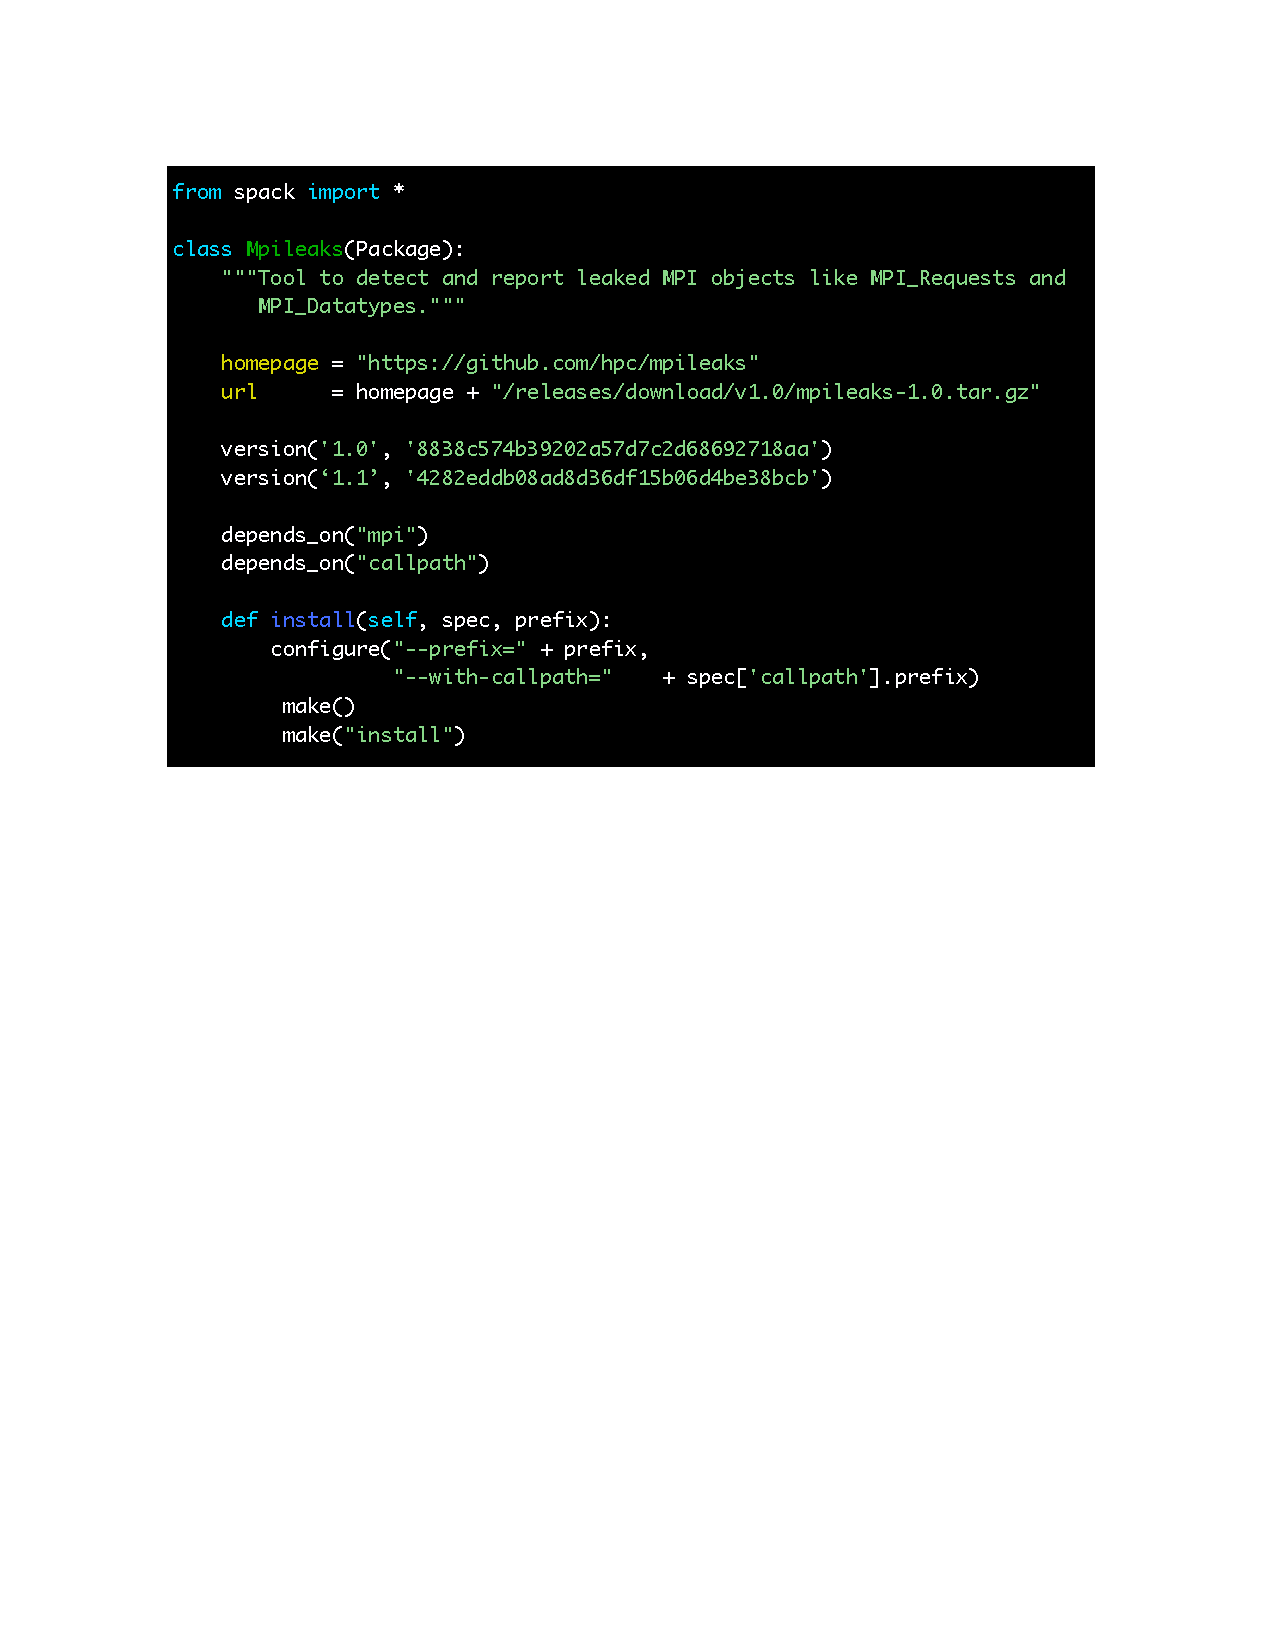
\includegraphics[width=\columnwidth]{code/mpileaks.pdf}
	\caption{
		Spack package for the {\tt mpileaks} tool.
		\label{fig:mpileaks}
	}
\end{figure}

Spack comprises many packages, and each describes how to build a software
artifact.  Each package is a class written in pure Python, but Spack uses
a simple, embedded domain-specific language (DSL) to make packaging easier.
Spack's DSL adds directives such as {\tt depends\_on}, {\tt version},
{\tt provides}, and {\tt extends}, in order to add metadata to package classes.

Figure~\ref{fig:mpileaks} shows the package for the \mpileaks tool.
Inside the {\tt MpiLeaks} class, the package provides a text description
and a homepage, as well as 
a download URL.  Notably, Spack packages can have {\it multiple} version
directives; each identifies a version and its checksum, allowing it to 
be downloaded and installed safely. Below this, three {\tt depends\_on}
directives indicate prerequisites that must be installed before \mpileaks.

\subsubsection{Installation Environment}



Existing package managers leave much up to package authors, and they 
frequently do
not always have 


Spack has a number of capabilities that make package writing more 
convenient. It can extrapolate a URL for each version using the {\tt url}
attribute as a model\footnote{This works for consistently named URLs,
and it can be specified per-version for packages with inconsistent naming.}.
It can use the same model to scrape webpages for new versions. 
Boilerplate for new packages can be generated from a URL.



Each package defines an {\tt install()} method, which is responsible
for its build. The {\tt install} environment is designed to look like
custom build scripts that LLNL staff have written for years.  Based on
past experience, we have tailored Spack's build environment to prevent common
build errors.

{\bf Familiar command syntax.} While Spack's Python DSL adds power and 
structure to the build process, LLNL staff are used to writing 
builds as shell scripts.  In Spack, shell commands can be invoked as
Python functions, which makes builds readable for package authors.
The {\tt mpileaks} build in Figure~\ref{fig:mpileaks} uses a 
shell-like installation procedure with it {\tt configure},
{\tt make}, and {\tt make install} calls.

{\bf Environment isolation.}
A common build error is to link in the wrong version of a library because
of an incorrect build environment.
%
For example, there are two versions of the {\tt libelf} library used by
LLNL performance tools. One is distributed with RedHat Linux, but the
publicly available version uses the same API but an incompatible ABI.
Failing to specify the right version can cause tools to crash.
%
Most build systems require users to manually specify paths to dependencies
installed in nonstandard locations.  This includes {\it most} software used
by HPC users.  However, depending on the package's particular build system,
libraries may be discovered
in different ways, either through special environment variables, compiler tests,
or manual specification in a Makefile or on the {\tt configure} line.

Spack manages the build environment by running each call to {\tt install}
in a new process.  This gives package authors full control of the build
process, and they can set build-specific environment variables without 
interfering with other packages.  It also helps packages find dependencies 
correctly, by setting
{\tt PATH}, {\tt PKG\_CONFIG\_PATH}, {\tt CMAKE\_PREFIX\_PATH}, and
{\tt LD\_LIBRARY\_PATH} to include the dependencies of the current build.
These variables are commonly used by build systems to locate dependencies,
and setting them ensures that incorrect libraries are not detected.

{\bf Compiler wrappers and RPATHs.}


The build scripts of existing packages managers are largely compiler-specific.
Most OS-specific package managers standardize on the same compiler used to build
the operating system, and offer some support for other compilers as an afterthought.
EasyBuild allows packages to be built with multiple toolchains, but it again
requires separate package files for each compiler.  Moreover, existing
package managers and LLNL's build scripts rely largely on package authors
to configure link options like {\tt RPATH}.  The setting is not enforced across
different packages, and enforcing a site-wide policy for link options is 
difficult.  If a package author forgets to add an {\tt RPATH}, the binary
can fail to run correctly.  Worse, a package maintainer may not detect this
after installing, because the package may work perfectly well in {\it her} 
environment but not that of other users.

Spack goes a step further and uses {\it compiler wrappers} to enforce
consistent link policies across builds.  



 a {\tt RPATHs} are ommitted

To make library finding more consistent, 

Also in the build environment, Spack sets the standard environment variables
{\tt CC}, {\tt CXX}, {\tt F77}, and {\tt FC} to point to custom compiler
wrapper scripts.  When run, the wrappers insert include ({\tt -I}), 
library ({\tt -L}), and {\tt RPATH} flags for all of the dependencies of
the package being built. This causes build tests like those in {\tt configure}
scripts to succeed.


These variables are used by most most modern build systems
to select the compilers to use for a build, so they are typically picked up
by default.

we must still add custom arguments to configuration scripts, as done for
{\tt callpath} and {\tt adept-utils} in Figure~\ref{fig:mpileaks}, but 

These environment
variables are respected by most modern build systems


 and {\tt -Wl,-rpath} flags 
aware of the location of the dependencies 



 will be invoked
after all of its prerequisites are built and installed.  takes the burden of
build consistency {\it off} of package authors by providing compiler 
wrappers that automatically set {\tt RPATHs} and guarantee that packages
find their dependencies.  Compiler wrappers also give package authors
more control over build options like compiler flags.

%The flags used to specify dependency locations are different from package
%to package, and build scripts frequently get these wrong.
%For example, in some LLNL packages that depend on the {\tt Silo} library,
%the {\tt --with-silo} parameter takes a path to {\tt Silo}'s prefix, but
%in others it takes both the {\tt include} and {\tt lib} subdirectories,
%separated by a comma.

\subsubsection{Potential for auto-generation of modules (with deps)}
	\todo{.5 page}



\begin{verbatim}
module disadvantages:
	- lmod solves a lot of problems
	- not on all systems
		- users often run from just a path.
		- not guaranteed that LD_LIBRARY_PATH, etc will
		  be set correctly.

- Lmod assumes build & submit environment must match
	- users often have NO IDEA what environment a package
	  was built with
	- multiple apps may be built with different stacks
	- combining them in a workflow is difficult with modules
		(need to know right incantation)

	- TACC implements a rather complicated mapping back to
	    the build env (Lmod CheckExec)
	

- Spack solves the matrix problem mentioned in the Lmod
    presentation (slide 98)
	- hierarchy is nasty -- every branch represents a
	  greedy choice
	- might NEED a specific version of ONE dependency
	  that is not supported in the tree
	  => SPACK!

- libmesh
	- boost, petsc, trilinos, grvy, etc.
\end{verbatim}

\subsection{Spack Specs}\label{sec:specs}

  Specs are partial descriptions of full
dependency graphs, but they are concise.  This allows a user to use
only a few parameters to quickly identify a configuration to install,
or to query existing installations and their dependencies.



\todo{1 page}



\subsection{Versioned Virtual Dependencies}
	\todo{.5 page}

\subsection{Abstract \& Concrete Specs}
	\todo{.75 page}
	

